%%
%% Copyright 2007, 2008, 2009 Elsevier Ltd
%%
%% This file is part of the 'Elsarticle Bundle'.
%% ---------------------------------------------
%%
%% It may be distributed under the conditions of the LaTeX Project Public
%% License, either version 1.2 of this license or (at your option) any
%% later version.  The latest version of this license is in
%%    http://www.latex-project.org/lppl.txt
%% and version 1.2 or later is part of all distributions of LaTeX
%% version 1999/12/01 or later.
%%
%% The list of all files belonging to the 'Elsarticle Bundle' is
%% given in the file `manifest.txt'.
%%

%% Template article for Elsevier's document class `elsarticle'
%% with numbered style bibliographic references
%% SP 2008/03/01
%%
%%
%%
%% $Id: elsarticle-template-num.tex 4 2009-10-24 08:22:58Z rishi $
%%
%%
\documentclass[12pt]{elsarticle}

%% Use the option review to obtain double line spacing
%% \documentclass[preprint,review,12pt]{elsarticle}

%% Use the options 1p,twocolumn; 3p; 3p,twocolumn; 5p; or 5p,twocolumn
%% for a journal layout:
%% \documentclass[final,1p,times]{elsarticle}
%% \documentclass[final,1p,times,twocolumn]{elsarticle}
%% \documentclass[final,3p,times]{elsarticle}
%% \documentclass[final,3p,times,twocolumn]{elsarticle}
%% \documentclass[final,5p,times]{elsarticle}
%% \documentclass[final,5p,times,twocolumn]{elsarticle}

%% if you use PostScript figures in your article
%% use the graphics package for simple commands
%% \usepackage{graphics}
%% or use the graphicx package for more complicated commands
\usepackage{graphicx}
%% or use the epsfig package if you prefer to use the old commands
%% \usepackage{epsfig}

%% The amssymb package provides various useful mathematical symbols
%\usepackage{amssymb}
%% The amsthm package provides extended theorem environments
%% \usepackage{amsthm}

%% The lineno packages adds line numbers. Start line numbering with
%% \begin{linenumbers}, end it with \end{linenumbers}. Or switch it on
%% for the whole article with \linenumbers after \end{frontmatter}.
%% \usepackage{lineno}

%% natbib.sty is loaded by default. However, natbib options can be
%% provided with \biboptions{...} command. Following options are
%% valid:

%%   round  -  round parentheses are used (default)
%%   square -  square brackets are used   [option]
%%   curly  -  curly braces are used      {option}
%%   angle  -  angle brackets are used    <option>
%%   semicolon  -  multiple citations separated by semi-colon
%%   colon  - same as semicolon, an earlier confusion
%%   comma  -  separated by comma
%%   numbers-  selects numerical citations
%%   super  -  numerical citations as superscripts
%%   sort   -  sorts multiple citations according to order in ref. list
%%   sort&compress   -  like sort, but also compresses numerical citations
%%   compress - compresses without sorting
%%
%% \biboptions{comma,round}

% \biboptions{}

\journal{Computational and Applied Mathematics}

\begin{document}

\begin{frontmatter}

%% Title, authors and addresses

%% use the tnoteref command within \title for footnotes;
%% use the tnotetext command for the associated footnote;
%% use the fnref command within \author or \address for footnotes;
%% use the fntext command for the associated footnote;
%% use the corref command within \author for corresponding author footnotes;
%% use the cortext command for the associated footnote;
%% use the ead command for the email address,
%% and the form \ead[url] for the home page:
%%

\title{A Set of difficulty Problems\\ for Testing Adaptive Finite Element Methods}

%% use optional labels to link authors explicitly to addresses:
\author[label1]{Zhonghua Ma}
\ead{mazhonghua83@gmail.com}
\author[label2]{Lukas Korous}
\ead{lukas.korous@gmail.com}
\author[label3]{Erick Santiago}
\ead{laviticus@sbcglobal.net}
\address[label1]{China University of Petroleum, Beijing, China}
\address[label2]{Charles University, Prague, Czech Republic}
\address[label3]{University of Nevada, Reno, USA}

\begin{abstract}
In this paper we provide a set of difficulties that can be used to
testing the ability of adaptive finite element algorithms to handle
a variety of types solutions. 
In each example we show sample results obtained with the
open source library {\sc Hermes}.\footnote{http://hpfem.org/hermes}
\end{abstract}

\begin{keyword}
Benchmark problem \sep Anisotropic solution \sep Test problems \sep $hp$-Finite element method
%% keywords here, in the form: keyword \sep keyword
%% MSC codes here, in the form: \MSC code \sep code
%% or \MSC[2008] code \sep code (2000 is the default)
\end{keyword}

\end{frontmatter}

%%
%% Start line numbering here if you want
%%
% \linenumbers

%% main text
\section{Introduction}
\label{sec:intro}

The number of adaptive finite element libraries is growing
-- let us mention (in alphabetical order) for example Alberta
\cite{alberta}, DealII \cite{dealii}, FEniCS
\cite{fenics}, FETK \cite{fetk}, Hermes \cite{hermes}, libMesh \cite{libmesh},
Phaml \cite{phaml}, PHG \cite{phg}, 2dhp90 \cite{2dhp90} and there are many others.\\
A natural question that arises is how do they compare to each other?
Unfortunately, comparison efforts are usually inhibited at the very beginning
by diverse installation requirements, supporting libraries, input and output
data formats, and different usage of various codes. And even if these problems
could be overcome, not many benchmarks with known exact solutions are
available to test various aspects of automatic adaptivity.
At this point we would like to acknowledge the pioneering work of Dr. William Mitchell
(NIST) who not only collected a suite of 12 benchmark problems
for adaptive FEM \cite{mitchell-1}, but who also implemented
and compared several $hp$-adaptive finite element algorithms by various
authors \cite{mitchell-2}.
This paper presents twelve parametrized test problems with different behaved 
solutions (contained in \cite{mitchell-1}) that are
designed to test the ability of adaptive algorithms.
The test problems and their
solutions are formulated in Sections \ref{sec:bench-1} - \ref{sec:bench-12}.
{\sc Hermes} is an open source C++ library for
rapid development of adaptive $hp$-FEM and $hp$-DG solvers.
In each section we show for illustration sample results obtained with the open
source {\sc Hermes} library (http://hpfem.org/hermes).

%%%%%%%%%%%%%%%%%%%%%%%%%%%%%%%%%%%%%%%%%%%%%%%%%%%%%%%%%%%%%%%%%%%%
\section{Benchmark NIST-1 "Analytic Solution"}
\label{sec:bench-1}
(NOTE:ALL figures in this paper will be update later!!)\\

This is the first benchmark problem with a smooth solution
that is used for testing how an adaptive algorithm behaves.
The equation solved is a Poisson equation

\begin{equation} \label{poisson}
-\Delta u = f
\end{equation}
in the domain $\Omega = (0, 1)^2$, equipped with Dirichlet
boundary condition given by the exact solution.
The exact solution $u(x, y) = 2^{4p}x^{p}(1-x)^{p}y^{p}(1-y)^{p}$
to this problem is shown in Fig. \ref{fig:sln-nist01}.
Here $p$ determines the degree of the polynomial solution.

\begin{figure}[!ht]
\centering
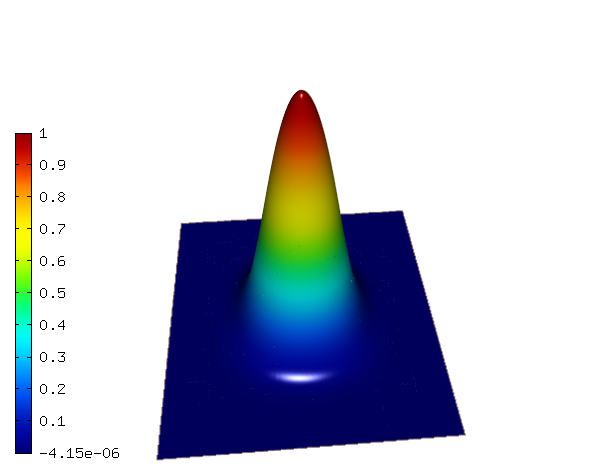
\includegraphics[height=5.5cm]{nist/nist-1/solution.png}
\caption{The solution to NIST-1 benchmark problem.}
\label{fig:sln-nist01}
\end{figure}
\noindent
The goal of the benchmark is to attain a relative error below
$10^{-2}$~\% in the $H^1$-norm with as few degrees of freedom (DOF)
as possible. 
We begin with adaptive $hp$-FEM with anisotropic refinements (adaptivity mode
HP\_ANISO in {\sc Hermes}). The initial mesh is shown in Fig. \ref{fig:nist-1-hp-aniso} (left).
In a few adaptivity steps, the polynomial degree of this element is increased
anisotropically.
The resulting mesh with 793 DOF is shown in Fig. \ref{fig:nist-1-hp-aniso} (right).

\begin{figure}[!ht]
\centering
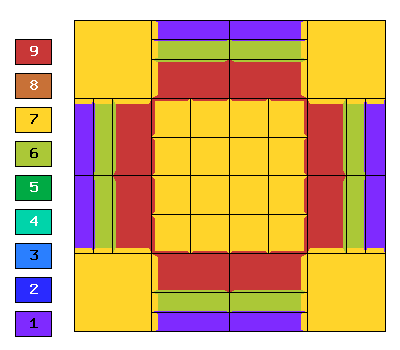
\includegraphics[height=5cm]{nist/nist-1/mesh_hp_anisoh.png}\ \
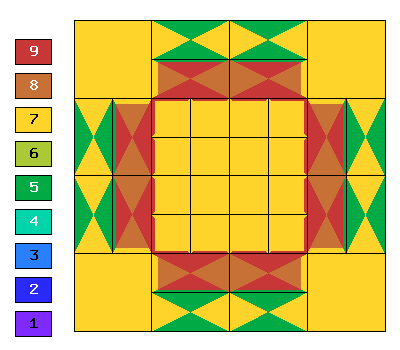
\includegraphics[height=5cm]{nist/nist-1/mesh_hp_aniso.png}
\vspace{-2mm}
\caption{Initial mesh (left) and final mesh (right) for $hp$-FEM with anisotropic refinements.}
\label{fig:nist-1-hp-aniso}
\end{figure}

The final relative error estimate in $H^1$-norm was 4.07698e-03 \%
and it was identical to the exact error in all printed digits.
We also solved this benchmark with adaptive $h$-FEM 
with linear (left) and quadratic (right)
elements, with anisotropic refinements enabled.
Final meshes for the $h$-FEM computations are shown 
in Fig. \ref{fig:nist-1-h-aniso}.

\begin{figure}[!ht]
\centering
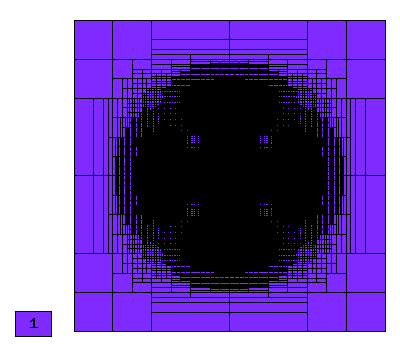
\includegraphics[height=5cm]{nist/nist-1/mesh_h1_aniso.png}\ \
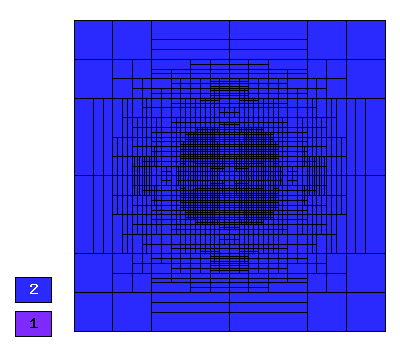
\includegraphics[height=5cm]{nist/nist-1/mesh_h2_aniso.png}
\vspace{-2mm}
\caption{Final mesh for $h$-FEM anisotropic refinements with linear and quadratic elements.}
\label{fig:nist-1-h-aniso}
\end{figure}
%\newpage

Figs. \ref{fig:nist-1-dof} and \ref{fig:nist-1-cpu} compare all
three adaptivity modes from the point
of view of DOF and CPU convergence.

\begin{figure}[!ht]
\centering
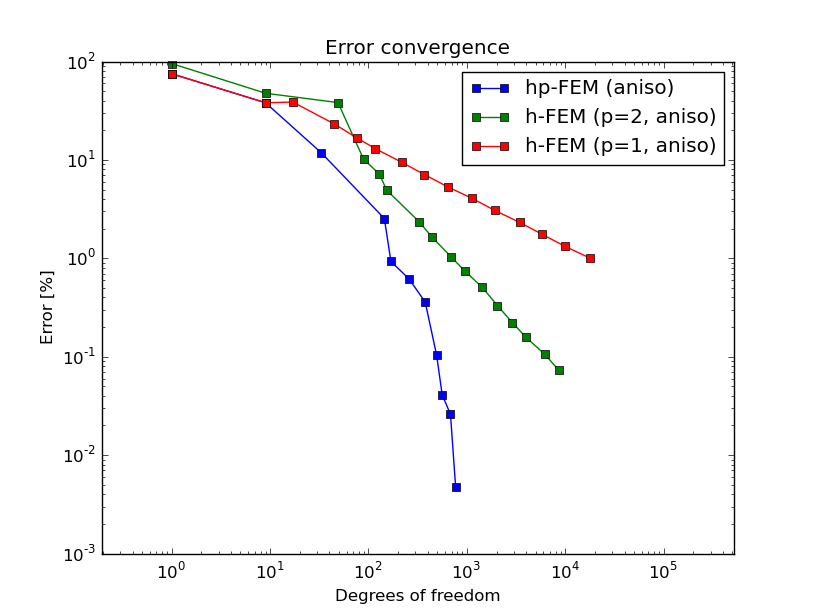
\includegraphics[height=5cm]{nist/nist-1/conv_dof_aniso.png}
\vspace{-2mm}
\caption{DOF convergence graphs.}
\label{fig:nist-1-dof}
\end{figure}

\begin{figure}[!ht]
\centering
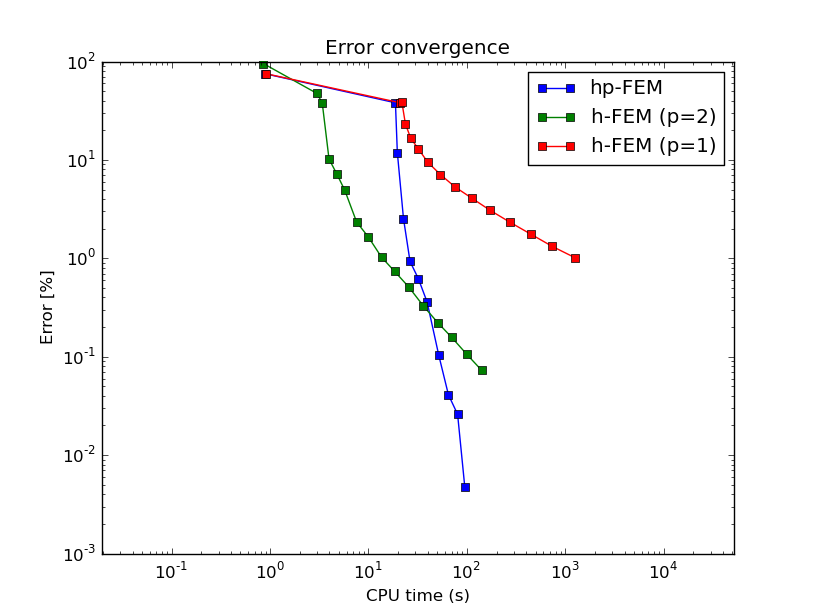
\includegraphics[height=5cm]{nist/nist-1/conv_cpu_aniso.png}
\vspace{-2mm}
\caption{CPU time convergence graphs.}
\label{fig:nist-1-cpu}
\end{figure}

%%%%%%%%%%%%%%%%%%%%%%%%%%%%%%%%%%%%%%%%%%%%%%%%%%%%%%%%%%%%%%%%%%%%
\section{Benchmark NIST-2 "Reentrant Corner"}
\label{sec:bench-2}

This is a standard benchmark for adaptive FEM algorithms.
The exact solution is smooth but contains singular gradient in a reentrant corner.
The equation solved is a Laplace equation

\begin{equation} \label{laplace}
-\Delta u = 0
\end{equation}
in the domain $\Omega = (-1, 1)^2$, with a section
removed from the clockwise side of positive $x$ axis.
Equation (\ref{laplace}) equipped with Dirichlet
boundary conditions given by the exact solution.

The exact solution
\begin{equation}\label{exact-nist-2}
u(x, y) = r^{\alpha}\sin(\alpha \theta)
\end{equation}
where $\alpha = \pi / \omega$, $r = \sqrt{x^2+y^2}$ and $\theta = tan^{-1}(y/x)$, here $\omega $ determines
the angle of the reentrant corner.
The solution of NIST-2 with $\omega = 3 \pi / 2$  is shown in Fig. \ref{fig:sln-nist02}.

\begin{figure}[!ht]
\centering
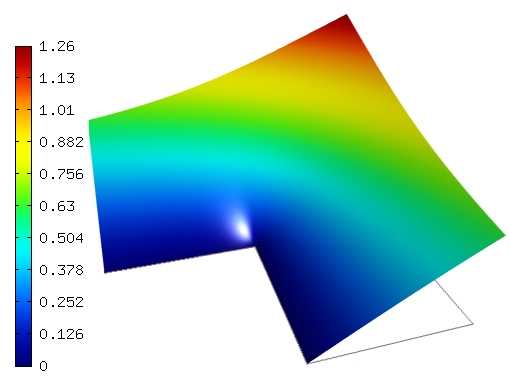
\includegraphics[height=6cm]{nist/nist-2/solution.png}
\caption{The solution to NIST-2 benchmark problem.}
\label{fig:sln-nist02}
\end{figure}

%%%%%%%%%%%%%%%%%%%%%%%%%%%%%%%%%%%%%%%%%%%%%%%%%%%%%%%%%%%%%%%%%%%%
\section{Benchmark NIST-3 "Linear Elasticity"}
\label{sec:bench-3}

This is a coupled system of two equations with a mixed
derivative for linear elasticity in the coupling term.

\begin{equation} \label{crack-u}
-E \frac{1-\nu^2}{1-2\nu} \frac{\partial^{2} u}{\partial x^{2}} - E\frac{1-\nu^2}{2-2 \nu} \frac{\partial^{2} u}{\partial y^{2}}
-E \frac{1-\nu^2}{(1-2\nu)(2-2\nu)} \frac{\partial^{2} v}{\partial x \partial y} = F_{x}
\end{equation}
\begin{equation} \label{crack-v}
-E \frac{1-\nu^2}{2-2\nu} \frac{\partial^{2} v}{\partial x^{2}} - E\frac{1-\nu^2}{1-2\nu} \frac{\partial^{2} v}{\partial y^{2}}
-E \frac{1-\nu^2}{(1-2\nu)(2-2\nu)} \frac{\partial^{2} u}{\partial x \partial y} = F_{y}
\end{equation}
where $F_{x} = F_{y} = 0$, $u$ and $v$ are the
$x$ and $y$ displacements, $E$ is Young's Modulus,
and $\nu$ is Poisson's ratio.

The domain is $\Omega = (0, 1)^2$, equipped with Dirichlet
boundary conditions given by the exact solution.

The exact solution
\begin{equation}\label{exact-nist-3-u-1}
u(x, y) = \frac{1}{2G} r^{\lambda}[(k - Q(\lambda + 1))cos(\lambda \theta) - \lambda cos((\lambda - 2) \theta)]
\end{equation}
\begin{equation}\label{exact-nist-3-v-1}
v(x, y) = \frac{1}{2G} r^{\lambda}[(k + Q(\lambda + 1))sin(\lambda \theta) + \lambda sin((\lambda - 2) \theta)]
\end{equation}
here $\lambda = 0.5444837367825$, $Q = 0.5430755788367$,
$k = 3 - 4 \nu$ and $G = E / (2(1 + \nu))$.

The solution of NIST-3 is shown in Fig. \ref{fig:sln-nist03-u} and Fig. \ref{fig:sln-nist03-v}.

\begin{figure}[!ht]
\centering
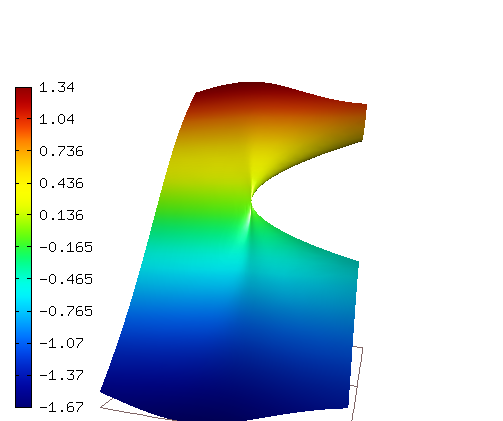
\includegraphics[height=6cm]{nist/nist-3/solution-u.png}
\caption{The $u$ component to NIST-3 benchmark problem.}
\label{fig:sln-nist03-u}
\end{figure}

\begin{figure}[!ht]
\centering
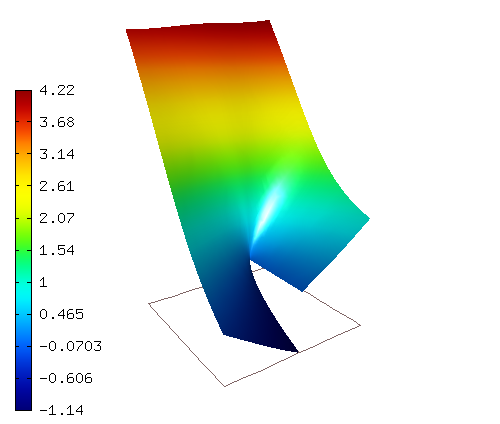
\includegraphics[height=6cm]{nist/nist-3/solution-v.png}
\caption{The $v$ component to NIST-3 benchmark problem.}
\label{fig:sln-nist03-v}
\end{figure}

%%%%%%%%%%%%%%%%%%%%%%%%%%%%%%%%%%%%%%%%%%%%%%%%%%%%%%%%%%%%%%%%%%%%
\section{Benchmark NIST-4 "Peak"}
\label{sec:bench-4}

This problem has an exponential peak in the interior of the domain.
The equation for this benchmark example is a Poisson equation

\begin{equation} \label{poisson-peak}
-\Delta u = f
\end{equation}
in the domain $\Omega = (0, 1)^2$, equipped with Dirichlet
boundary conditions given by the exact solution.

The exact solution
\begin{equation}\label{exact-nist-4}
u(x,y) = e^{-\alpha ((x - x_{loc})^{2} + (y - y_{loc})^{2})}
\end{equation}
where $(x_{loc}, y_{loc})$ is the location of the peak,
$\alpha$ determines the strength of the peak.
The right-hand side $f$ is calculated by inserting (\ref{exact-nist-4}) into (\ref{poisson-peak}).
The solution of NIST-4 with $\alpha = 1000$, $(x_{loc}, y_{loc}) = (0.5, 0.5)$ is shown in Fig. \ref{fig:sln-nist04}.

\begin{figure}[!ht]
\centering
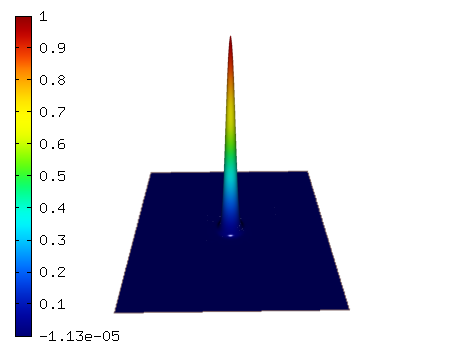
\includegraphics[height=6cm]{nist/nist-4/solution.png}
\caption{The solution to NIST-4 benchmark problem.}
\label{fig:sln-nist04}
\end{figure}

%%%%%%%%%%%%%%%%%%%%%%%%%%%%%%%%%%%%%%%%%%%%%%%%%%%%%%%%%%%%%%%%%%%%
\section{Benchmark NIST-5 "Battery"}
\label{sec:bench-5}

This is a heat conduction problem in a nonhomogeneous material. It comes with an anisotropic solution and
multiple singularities. The solution has multiple point singularities in the interior of the domain.
The equation is given below

\begin{equation} \label{heat-conduction}
-\frac{\partial }{\partial x}\left(p(x, y)\frac{\partial u}{\partial x}\right)
-\frac{\partial }{\partial y}\left(q(x, y)\frac{\partial u}{\partial y}\right) = f
\end{equation}
in the domain $\Omega = (0, 8.4) \times (0, 24)$, equipped with
a zero Neumann boundary condition on left edge, Natural boundary conditions on the rest of the boundary.

\begin{equation}
p(x, y)\frac{\partial u}{\partial x}\nu_1 + q(x, y)\frac{\partial u}{\partial y}\nu_2 = g_{left}(x, y) \ \mbox{on} \  \Gamma_{left}
\end{equation}

\begin{equation}
p(x, y)\frac{\partial u}{\partial x}\nu_1 + q(x, y)\frac{\partial u}{\partial y}\nu_2 + c(x, y)u = g_{right}(x, y) \ \mbox{on} \ \Gamma_{right}
\end{equation}

\begin{equation}
p(x, y)\frac{\partial u}{\partial x}\nu_1 + q(x, y)\frac{\partial u}{\partial y}\nu_2 + c(x, y)u = g_{top}(x, y) \ \mbox{on} \ \Gamma_{top}
\end{equation}

\begin{equation}
p(x, y)\frac{\partial u}{\partial x}\nu_1 + q(x, y)\frac{\partial u}{\partial y}\nu_2 + c(x, y)u = g_{bottom}(x, y) \ \mbox{on} \ \Gamma_{bottom}
\end{equation}
where $p(x, y)$, $q(x, y)$, $c(x, y)$, $g(x, y)$
and the right hand side $f$ are constant coefficient
functions in different materials.

The solution of NIST-5 is shown in Fig. \ref{fig:sln-nist05}.
\begin{figure}[!ht]
\centering
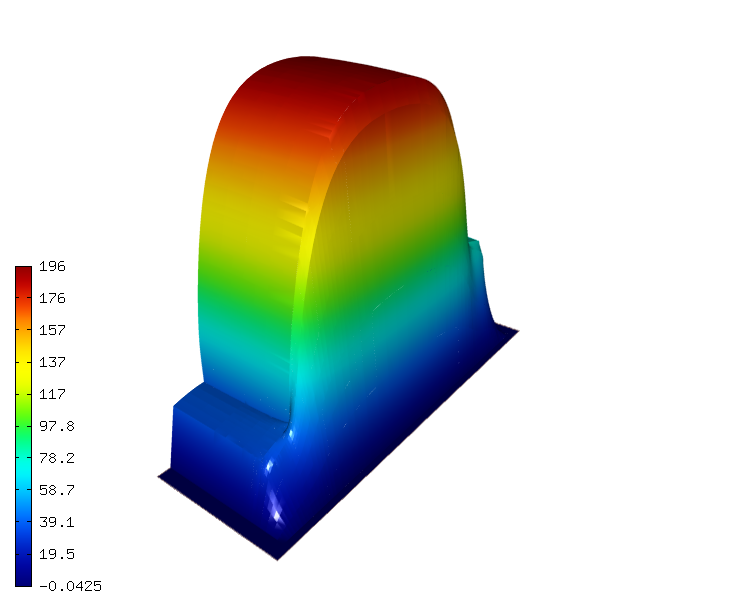
\includegraphics[height=6cm]{nist/nist-5/solution-3d.png}
\caption{The solution to NIST-5 benchmark problem.}
\label{fig:sln-nist05}
\end{figure}

%%%%%%%%%%%%%%%%%%%%%%%%%%%%%%%%%%%%%%%%%%%%%%%%%%%%%%%%%%%%%%%%%%%%
\section{Benchmark NIST-6 "Boundary Layer"}
\label{sec:bench-6}

This problem has an boundary layer along the right and top sides of the domain.
It is a convection-diffusion equation with first order terms.

\begin{equation} \label{boundary-layer}
-\epsilon \nabla^{2} u + 2\frac{\partial u}{\partial x} + \frac{\partial u}{\partial y}= f
\end{equation}
in the domain $\Omega = (-1, 1)^2$, equipped with Dirichlet boundary condition
given by the exact solution.

The exact solution
\begin{equation}\label{exact-nist-6}
u(x,y) = (1 - e^{-(1 - x) / \epsilon})(1 - e^{-(1 - y) / \epsilon})cos(\pi (x + y))
\end{equation}
where $\epsilon$ determines the strength of the boundary layer.
The right-hand side $f$ is calculated by inserting (\ref{exact-nist-6}) into (\ref{boundary-layer}).
The solution of NIST-6 with $\epsilon = 10^{-1}$ is shown in Fig. \ref{fig:sln-nist06}.

\begin{figure}[!ht]
\centering
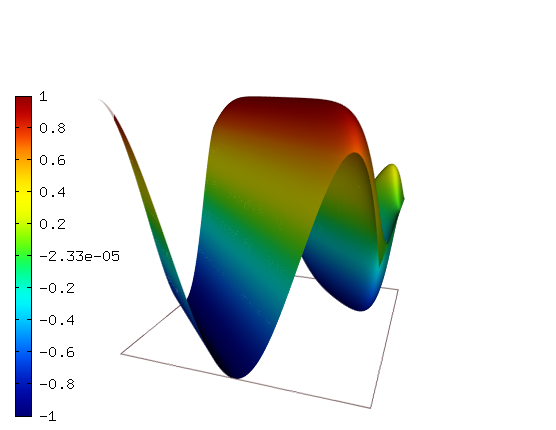
\includegraphics[height=6cm]{nist/nist-6/solution.png}
\caption{The solution to NIST-6 benchmark problem.}
\label{fig:sln-nist06}
\end{figure}

%%%%%%%%%%%%%%%%%%%%%%%%%%%%%%%%%%%%%%%%%%%%%%%%%%%%%%%%%%%%%%%%%%%%
\section{Benchmark NIST-7 "Boundary Line Singularity"}
\label{sec:bench-7}

This is a singularity problem with a solution that is singular along the left boundary.
The equation of this problem is Poisson equation

\begin{equation} \label{boundary-line-singularity}
-\Delta u = f
\end{equation}
in the domain $\Omega = (0, 1)^2$, equipped with Dirichlet boundary conditions
given by the exact solution.

The exact solution
\begin{equation}\label{exact-nist-7}
u(x,y) = x^{\alpha}
\end{equation}
where $\alpha \geq 0.5$ determines the strength of the singularity.
The right-hand side $f$ is calculated by inserting (\ref{exact-nist-7}) into (\ref{boundary-line-singularity}).
The solution of NIST-7 with $\alpha = 0.6$ is shown in Fig. \ref{fig:sln-nist07}.

\begin{figure}[!ht]
\centering
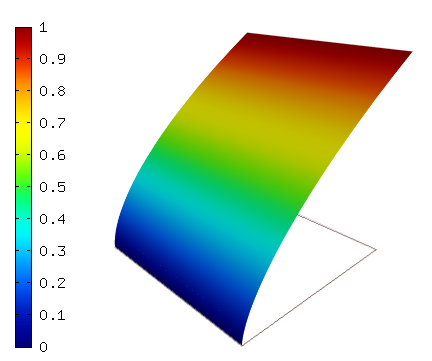
\includegraphics[height=6cm]{nist/nist-7/solution.png}
\caption{The solution to NIST-7 benchmark problem.}
\label{fig:sln-nist07}
\end{figure}

%%%%%%%%%%%%%%%%%%%%%%%%%%%%%%%%%%%%%%%%%%%%%%%%%%%%%%%%%%%%%%%%%%%%
\section{Benchmark NIST-8 "Oscillatory"}
\label{sec:bench-8}

This is a wave function that satisfies a Schrodinger equation model of two
interacting atoms with highly oscillatory near the origin.
The equation resolved is

\begin{equation} \label{oscillatory}
-\nabla^{2} u - \frac{1}{(\alpha + r)^{4}} u = f
\end{equation}
in the domain $\Omega = (0, 1)^2$, equipped with Dirichlet boundary conditions
given by the exact solution.

The exact solution
\begin{equation}\label{exact-nist-8}
u(x,y) = sin(\frac{1}{\alpha + r})
\end{equation}
where $r = \sqrt{x^{2} + y^{2}}$, $\alpha = \frac{1}{N \pi}$ determines the number of oscillations.
The right-hand side $f$ is calculated by inserting (\ref{exact-nist-8}) into (\ref{oscillatory}).
The solution of NIST-8 with $\alpha = \frac{1}{10 \pi}$ is shown in Fig. \ref{fig:sln-nist08}.

\begin{figure}[!ht]
\centering
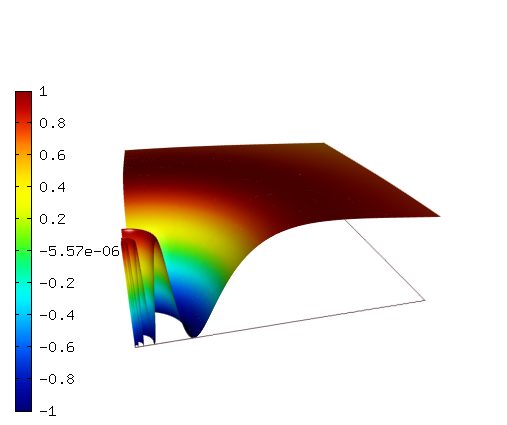
\includegraphics[height=6cm]{nist/nist-8/solution.png}
\caption{The solution to NIST-8 benchmark problem.}
\label{fig:sln-nist08}
\end{figure}

%%%%%%%%%%%%%%%%%%%%%%%%%%%%%%%%%%%%%%%%%%%%%%%%%%%%%%%%%%%%%%%%%%%%
\section{Benchmark NIST-9 "Wave Front"}
\label{sec:bench-9}

This is a standard benchmark for adaptive FEM algorithms.The exact solution is smooth
but contains singular gradient in a re-entrant corner.
The equation solved is a Poisson equation

\begin{equation} \label{wave-front}
-\Delta u = f
\end{equation}
in the domain $\Omega = (0, 1)^2$, equipped with Dirichlet boundary conditions
given by the exact solution.

The exact solution
\begin{equation}\label{exact-nist-9}
u(x, y) = tan^{-1}(\alpha (r - r_{0}))
\end{equation}
where $r = \sqrt{(x - x_{loc})^{2} + (y - y_{loc})^{2}}$,
here $(x_{loc}, y_{loc})$ is the center of the circular wave front,
$r_{0}$ is the distance from the wave front to the center of the circle,
and $\alpha$ gives the steepness of the wave front.
The right-hand side $f$ is calculated by inserting (\ref{exact-nist-9}) into (\ref{wave-front}).
The solution of NIST-9 with $\alpha = 50$, $(x_{loc}, y_{loc}) = (0.5, 0.5)$,
$r_{0} = 0.25$ is shown in Fig. \ref{fig:sln-nist09}.

\begin{figure}[!ht]
\centering
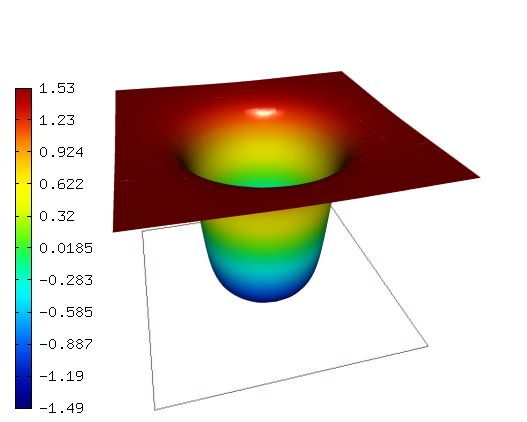
\includegraphics[height=6cm]{nist/nist-9/solution.png}
\caption{The solution to NIST-9 benchmark problem.}
\label{fig:sln-nist09}
\end{figure}

%%%%%%%%%%%%%%%%%%%%%%%%%%%%%%%%%%%%%%%%%%%%%%%%%%%%%%%%%%%%%%%%%%%%
\section{Benchmark NIST-10 "Interior Line Singularity"}
\label{sec:bench-10}

This is another example with anisotropic solution that is suitable for testing
anisotropic element refinements.
The equation solved is a Poisson equation

\begin{equation} \label{interior}
-\Delta u = f
\end{equation}
in the domain $\Omega = (-1, 1)^2$, equipped with a zero
Neumann boundary condition on left edge, Dirichlet boundary conditions given by the
exact solution on the rest of the boundary.

The exact solution
\begin{equation}\label{exact-nist-10-1}
u(x,y) = \cos(Ky)\ \ \ \mbox{for}\ x \le 0
\end{equation}
\begin{equation}\label{exact-nist-10-2}
u(x,y) = \cos(Ky) + x^{\alpha}\ \ \ \mbox{for}\ x > 0
\end{equation}
where $K$ and $\alpha$ are real constants.
The right-hand side $f$ is calculated by inserting
(\ref{exact-nist-10-1}) and (\ref{exact-nist-10-2}) into (\ref{wave-front}).
The solution of NIST-10 with $K = \pi/2$ and
$\alpha = 2.01$ is shown in Fig. \ref{fig:sln-nist10}.

\begin{figure}[!ht]
\centering
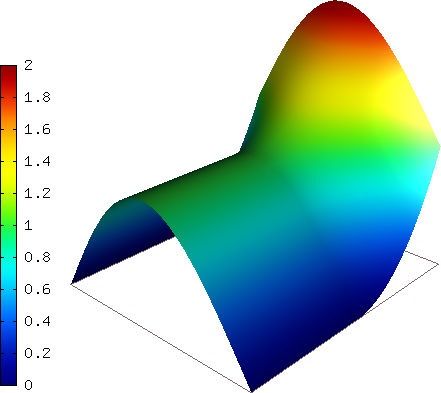
\includegraphics[height=6cm]{nist/nist-10/solution.png}
\caption{The solution to NIST-10 benchmark problem.}
\label{fig:sln-nist10}
\end{figure}

%%%%%%%%%%%%%%%%%%%%%%%%%%%%%%%%%%%%%%%%%%%%%%%%%%%%%%%%%%%%%%%%%%%%
\section{Benchmark NIST-11 "Intersecting Interfaces"}
\label{sec:bench-11}

The solution to this elliptic problems contains a severe
singularity that poses a challenge to adaptive methods.
The equation is given as below

\begin{equation} \label{intersecting}
-\nabla \cdot (a(x,y) \nabla u) = 0
\end{equation}
where the parameter $a$ is piecewise-constant,
$a(x,y) = R$ in the first and third quadrants
and $a(x,y) = 1$ in the remaining two quadrants.
The domain of this problem is $\Omega = (-1, 1)^2$, equipped with
Dirichlet boundary conditions given by the exact solution.

The exact solution
\begin{equation}\label{exact-nist-11}
u(x,y) = r^{a} \mu
\end{equation}

The solution of NIST-11 is shown in Fig. \ref{fig:sln-nist11}.

\begin{figure}[!ht]
\centering
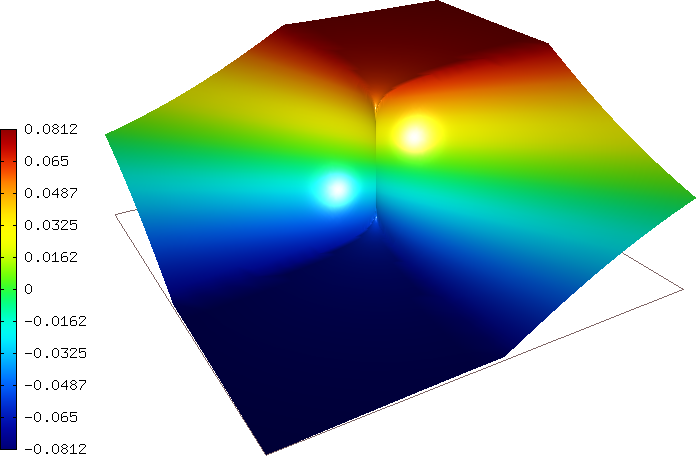
\includegraphics[height=6cm]{nist/nist-11/solution.png}
\caption{The solution to NIST-11 benchmark problem.}
\label{fig:sln-nist11}
\end{figure}


%%%%%%%%%%%%%%%%%%%%%%%%%%%%%%%%%%%%%%%%%%%%%%%%%%%%%%%%%%%%%%%%%%%%
\section{Benchmark NIST-12 "Multiple Difficulties"}
\label{sec:bench-12}

The solution to this elliptic problems contains four difficulties
of different strengths into the same problem
(nist-2, nist-4, nist-6 and nist-9).
The equation solved is a Poisson equation

\begin{equation} \label{multiple}
-\Delta u = f
\end{equation}
in the L-shaped domain, equipped with Dirichlet boundary conditions
given by the exact solution.

The exact solution
\begin{equation}\label{exact-nist-12}
u(x,y) =  r^{\alpha_{C} }\sin(\alpha_{C} \theta)
+ e^{-\alpha_{P} ((x - x_{P})^{2} + (y - y_{P})^{2})}
+ tan^{-1}(\alpha_{W} (r_{W} - r_{0}))
+ e^{-(1 - y) / \epsilon}
\end{equation}
where $\alpha_C = \pi / \omega_C$, $r = \sqrt{x^2+y^2}$
and $\theta = tan^{-1}(y/x)$, here $\omega_C$ determines
the angle of the re-entrant corner.
$(x_{P}, y_{P})$ is the location of the peak, $\alpha$
determines the strength of the peak.
$r_{W} = \sqrt{(x - x_{W})^{2} + (y - y_{W})^{2}}$,
here $(x_{W}, y_{W})$ is the center of the circular wave front,
$r_{0}$ is the distance from the wave front to the
center of the circle, and $\alpha_W$ gives
the steepness of the wave front. $\epsilon$ determines the
strength of the boundary layer, the boundary layer was placed on $y = -1$.
The right-hand side $f$ is calculated by inserting (\ref{exact-nist-12})
into (\ref{multiple}). \\

The solution of NIST-12 with $\omega_C = 3 \pi /2$,
$(x_{W}, y_{W}) = (0, -3/4)$, $r_{0} = 3/4$, $\alpha_{W} = 200$,
$(x_{P}, y_{P}) = (\sqrt{5} / 4, -1/4)$,
$\epsilon = 1/100$ is shown in Fig. \ref{fig:sln-nist12}.

\begin{figure}[!ht]
\centering
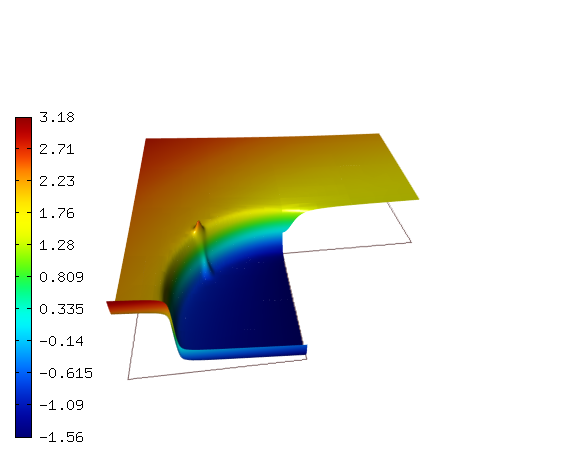
\includegraphics[height=6cm]{nist/nist-12/solution.png}
\caption{The solution to NIST-12 benchmark problem.}
\label{fig:sln-nist12}
\end{figure}

%%%%%%%%%%%%%%%%%%%%%%%%%%%%%%%%%%%%%%%%%%%%%%%%%%%%%%%%%%%%%%%%%%%%
\section{Conclusion and Outlook}
\label{sec:conclusion}

%We have presented three new benchmark problems with known exact solutions
%that can be used to assess the ability of adaptive FEM codes to handle
%anisotropic refinements. Since for adaptive FEM codes the resulting mesh
%should be observed as part of the final solution, we are currently expanding
%our research of optimal meshes.

\section{Acknowledgment}

This work was supported by Subcontract No. 00089911 of Battelle
Energy Alliance (DOE intermediary) as well as by the
Grant No. IAA100760702 of the Grant Agency of the Academy
of Sciences of the Czech Republic. The first autor was partly
supported by the National Natural Science Foundation
of China under Projects No. 41074099.

%
%
%\appendix
%\section{Sample Results Obtained with {\sc Hermes}}\label{sec:app}
%
%In the second part of this paper we provide sample solutions to
%the above benchmark problems using the {\sc Hermes} library.
%The results are provided for illustration purposes only and they
%should not be used as reference values.
%
%
%\subsection*{Brief Description of the {\sc Hermes} Library}
%{\sc Hermes} is an open source C++ library for
%rapid development of adaptive $hp$-FEM and $hp$-DG solvers. The library is
%developed by the $hp$-FEM group at the University of Nevada, Reno
%(http://hpfem.org) and it is available under the GPL license.
%
%{\sc Hermes} offers eight different modes of automatic adaptivity:
%\begin{enumerate}
%\item H\_ISO ($h$-adaptivity with isotropic refinements),
%\item H\_ANISO ($h$-adaptivity with possibly anisotropic refinements),
%\item P\_ISO ($p$-adaptivity with isotropic polynomial degrees in elements),
%\item P\_ANISO ($p$-adaptivity with possibly anisotropic polynomial degrees in elements),
%\item HP\_ISO ($hp$-adaptivity with isotropic polynomial degrees in elements and isotropic spatial refinements),
%\item HP\_ANISO\_H ($hp$-adaptivity with isotropic polynomial degrees in elements and possibly anisotropic spatial refinements),
%\item HP\_ANISO\_P ($hp$-adaptivity with possibly anisotropic polynomial degrees in elements and isotropic spatial refinements),
%\item HP\_ANISO ($hp$-adaptivity with possibly anisotropic polynomial degrees in elements and possibly anisotropic spatial refinements).
%\end{enumerate}
%
%\subsection*{Main Idea of the Adaptivity Algorithm}
%
%In each adaptivity step the algorithm performs a global $hp$ mesh refinement,
%calculates an approximate (reference) solution $u_{ref}$ on the refined mesh, obtains its
%closest representant $u_{coarse}$ on the original coarse mesh via an orthogonal projection,
%and evaluates the approximate error function
%$$
%e_{h,p} = u_{ref} - u_{coarse}.
%$$
%In fact, $u_{coarse}$ is the low-order part of $u_{ref}$ and so $e_{h,p}$
%is an excellent indicator where $u_{coarse}$ needs to be improved.
%Next, the algorithm identifies elements with the largest error norm,
%and selects them for refinement. Last, in a loop over all selected
%elements $K$, the algorithm projects $u_{ref}$ locally on all refinement
%candidates on $K$. Here is where the various adaptivity modes differ --
%the simplest one is H\_ISO with just one refinement option (a 4-split) and mode
%8 is the most general with around 100 options. This looks like lots of
%CPU time, but in reality the projections are extremely
%fast since each refinement candidate comes with a local orthonormal basis.
%Among all considered refinements of $K$, the algorithm select the one
%which yields the smallest projection error (weighted with the number of
%new degrees of freedom that the candidate adds to the discrete problem).
%
%The algorithm is completely PDE-independent, it does not contain
%any tuning parameters, and in contrast to various popular gradient-based techniques
%it works equally well for low-order and high-order elements. Thanks to its
%robustness and simplicity, the algorithm works
%very well for multiphysics PDE systems where it is used in combination
%with multimesh $hp$-FEM \cite{thermoel}.
%
%\subsection*{Benchmark No. 1}
%
%We begin with adaptive $hp$-FEM with anisotropic refinements (adaptivity mode
%HP\_ANISO in {\sc Hermes}), starting from a mesh that contains only one bilinear
%element. The initial mesh is shown in Fig. \ref{fig:1-hp-aniso} (left).
%In a few adaptivity steps, the polynomial degree of this element is increased
%anisotropically and the element is never refined in space.
%The resulting single-element mesh with 16 DOF is shown in Fig. \ref{fig:1-hp-aniso} (right). The diagonal pattern
%indicates different polynomial degrees ($8$ in the $x$-direction and $1$ in the $y$-direction).
%
%\newpage
%
%\begin{figure}[!ht]
%\centering
%\includegraphics[height=5cm]{solinfig5.eps}\ \
%\includegraphics[height=5cm]{solinfig6.eps}
%\caption{Initial mesh (left) and final mesh (right) for $hp$-FEM with anisotropic refinements.}
%\label{fig:1-hp-aniso}
%\end{figure}
%
%The final relative error estimate in $H^1$-norm was 3.6796e-05 \%
%and it was identical to the exact error in all printed digits.
%
%We also solved this benchmark with adaptive $h$-FEM with quadratic
%elements, with anisotropic refinements enabled and disabled
%(adaptivity modes H\_ANISO and H\_ISO in {\sc Hermes}, respectively).
%Final meshes for the $h$-FEM computations are not shown here --
%they were so fine that they appeared as black squares. The $h$-FEM
%with isotropic refinements was stopped after reaching 100,000 DOF.
%Figs. \ref{fig:1-graph-1} and \ref{fig:1-graph-2} compare all
%three adaptivity modes from the point
%of view of DOF and CPU convergence.
%
%\begin{figure}[!ht]
%\centering
%\includegraphics[height=7cm]{solinfig7.eps}
%\vspace{-2mm}
%\caption{DOF convergence graphs.}
%\label{fig:1-graph-1}
%\vspace{-1cm}
%\end{figure}
%\newpage
%
%\begin{figure}[!ht]
%\centering
%\includegraphics[height=7cm]{solinfig8.eps}
%\vspace{-2mm}
%\caption{CPU time convergence graphs.}
%\label{fig:1-graph-2}
%\end{figure}
%
%
%\subsection*{Benchmark No. 2}
%
%First we employ $hp$-FEM with anisotropic refinements (HP\_ANISO mode in {\sc Hermes})
%and start from a 100-element
%mesh that was obtained through several consecutive refinements towards
%the boundary. Note that herewith we use some a-priori knowledge of the
%solution. The initial mesh and the final mesh with 3,913 DOF
%are shown in the left and right part of Fig. \ref{fig:2-hp-aniso}, respectively.
%
%\begin{figure}[!ht]
%\centering
%\includegraphics[height=5cm]{solinfig9.eps}\ \
%\includegraphics[height=5cm]{solinfig10.eps}
%\caption{Initial mesh (left) and final mesh (right) for $hp$-FEM with anisotropic refinements.}
%\label{fig:2-hp-aniso}
%\end{figure}
%\noindent
%
%We also solved this benchmark using adaptive $h$-FEM with quadratic
%elements, with anisotropic refinements enabled and disabled (adaptivity
%modes H\_ANISO and H\_ISO in {\sc Hermes}, respectively). The
%corresponding final meshes are shown in Fig. \ref{fig:2-h2}.
%
%\begin{figure}[!ht]
%\centering
%\includegraphics[height=5cm]{solinfig11.eps}\ \
%\includegraphics[height=5cm]{solinfig12.eps}
%\caption{Resulting meshes for $h$-FEM with quadratic elements. Anisotropic
%   refinements enabled (left) and disabled (right).}
%\label{fig:2-h2}
%\end{figure}
%\noindent
%
%Again, computations were stopped when the number of DOF exceeded 100,000.
%Figs. \ref{fig:2-graph-1} and  \ref{fig:2-graph-2} compare all
%three adaptivity modes from the point of view of DOF and CPU time convergence.
%
%\begin{figure}[!ht]
%\centering
%\includegraphics[height=7cm]{solinfig13.eps}
%\vspace{-2mm}
%\caption{DOF convergence graphs. }
%\label{fig:2-graph-1}
%\end{figure}
%
%\newpage
%
%\begin{figure}[!ht]
%\centering
%\includegraphics[height=7cm]{solinfig14.eps}
%\vspace{-2mm}
%\caption{CPU time convergence graphs.}
%\label{fig:2-graph-2}
%\vspace{-0.5cm}
%\end{figure}
%
%\subsection*{Benchmark No. 3}
%
%As in the previous two cases, we begin with $hp$-FEM with anisotropic refinements
%(HP\_ANISO mode in {\sc Hermes}). The initial mesh for the first solution component
%is just one quadratic element and the initial mesh for the second component
%has 100 quadratic elements, as shown in Fig. \ref{fig:3-init}
%
%\begin{figure}[!ht]
%\centering
%\includegraphics[height=5cm]{solinfig15.eps}\ \
%\includegraphics[height=5cm]{solinfig16.eps}
%\caption{Initial meshes for the two solution components.}
%\label{fig:3-init}
%\end{figure}
%\noindent
%
%The final meshes for the first and second solution components
%are shown in Fig. \ref{fig:3-hp-aniso}. They contain 49 and
%1,809 DOF, respectively (total of 1,858 DOF).
%
%\begin{figure}[!ht]
%\centering
%\includegraphics[height=5cm]{solinfig17.eps}\ \
%\includegraphics[height=5cm]{solinfig18.eps}
%\caption{Final meshes for both solution components, $hp$-FEM with
%         anisotropic refinements.}
%\label{fig:3-hp-aniso}
%\end{figure}
%\noindent
%
%Again we also solved this benchmark using adaptive $h$-FEM with quadratic
%elements, with anisotropic refinements enabled and disabled (adaptivity
%modes H\_ANISO and H\_ISO in {\sc Hermes}, respectively). The
%corresponding final meshes for the anisotropic case are shown in
%Fig. \ref{fig:3-h2-aniso}. They contain 4,961 DOF and 49,873 DOF
%(total of 54,834 DOF).
%
%\begin{figure}[!ht]
%\centering
%\includegraphics[height=5cm]{solinfig19.eps}\ \
%\includegraphics[height=5cm]{solinfig20.eps}
%\caption{Final meshes for both solution components, $h$-FEM with
%         quadratic elements and anisotropic refinements enabled.}
%\label{fig:3-h2-aniso}
%\end{figure}
%
%\clearpage
%
%\noindent
%The final meshes for the isotropic case are shown in Fig.
%\ref{fig:3-h2-iso}. They contain 961 DOF and 81,185, DOF
%(total of 82,146, DOF).
%
%\begin{figure}[!ht]
%\centering
%\includegraphics[height=5cm]{solinfig21.eps}\ \
%\includegraphics[height=5cm]{solinfig22.eps}
%\caption{Final meshes for both solution components, $h$-FEM with
%         quadratic elements and isotropic refinements.}
%\label{fig:3-h2-iso}
%\end{figure}
%
%
%Also in this case computations were stopped when the number of DOF exceeded 100,000.
%Figs. \ref{fig:3-graph-1} and  \ref{fig:3-graph-2} compare all
%three adaptivity modes from the point of view of DOF and CPU time convergence.
%
%\begin{figure}[!ht]
%\centering
%\includegraphics[height=7cm]{solinfig23.eps}
%\vspace{-2mm}
%\caption{DOF convergence graphs. }
%\label{fig:3-graph-1}
%\end{figure}
%
%
%\begin{figure}[!ht]
%\centering
%\includegraphics[height=7cm]{solinfig24.eps}
%\vspace{-2mm}
%\caption{CPU time convergence graphs.}
%\label{fig:3-graph-2}
%\end{figure}
%
%







\begin{thebibliography}{[KLR73]}
%
% and use \bibitem to create references.
%
% Use the following syntax and markup for your references
%
% Monographs

\bibitem{label1}
D. Estep, G. Carey, V. Ginting, S. Tavener, T. Wildey:
A Posteriori Error Analysis of Multiscale Operator
Decomposition Methods for Multiphysics Models, SciDAC 2008,
Journal of Physics: Conference Series 125 (2008) 12 - 75.

\bibitem{fitzhugh}
R. Fitzhugh: Mathematical Models of Excitation and Propagation in Nerve.
Chapter 1, pp. 1-85 in H.P. Schwan, ed. Biological Engineering,
McGraw-Hill Book Co., N.Y. (1969).

\bibitem{mitchell-1}
W. Mitchell: A Collection of 2D Elliptic Problems for
Testing Adaptive Algorithms, NISTIR 7668, 2010 (available online).

\bibitem{mitchell-2}
W. Mitchell: A Survey of hp-Adaptive Strategies for Elliptic Partial Differential Equations,
Annals of the European Academy of Sciences, to appear (available online).

\bibitem{nagumo}
J. Nagumo, S. Arimoto, S. Yoshizawa:
An Active Pulse Transmission Line Simulating Nerve Axon. Proc. IRE 50, 2061–2070 (1962).

\bibitem{label2}
P. Solin, D. Andrs, J. Cerveny, M. Simko:
PDE-Independent Adaptive $hp$-FEM Based on Hierarchic Extension of Finite Element Spaces.
J. Comput. Appl. Math. 233 (2010) 3086-3094.


\bibitem{thermoel}
P. Solin, J. Cerveny, L. Dubcova, D. Andrs:
Monolithic Discretization of Linear Thermoelasticity Problems
via Adaptive Multimesh $hp$-FEM, J. Comput. Appl. Math 234 (2010) 2350 - 2357.

\bibitem{sosedo}
P. Solin. K. Segeth, I. Dolezel: Higher-Order Finite Element Methods, Chapman \& Hall
/ CRC Press, Boca Raton, 2003.

% Contributed Works
%\bibitem[Mey89]{contribution} Meyer, P.A.: A short presentation of
%stochastic calculus. In: Emery, M. (ed) Stochastic Calculus in
%Manifolds. Springer, Berlin Heidelberg New York (1989)
%
% Journal
%\bibitem[MR97]{journal} Miller, B.M., Runggaldier, W.J.: Kalman
%filtering for linear systems with coefficients driven by a hidden Markov
%jump process. Syst. Control Lett., \textbf{31}, 93--102 (1997)
%
% Theses
%\bibitem[Ros77]{thesis} Ross, D.W.: Lysosomes and storage diseases. MA
%Thesis, Columbia University, New York (1977)

\end{thebibliography}

\vbox{}
\vspace{6mm}
We also include online references to the FEM codes mentioned in this paper.
All these URLs were active on September 30, 2010:

\begin{thebibliography}{[codes]}

\bibitem{alberta}
Alberta: http://www.alberta-fem.de/

\bibitem{dealii}
DealII (Differential Equations Analysis Library) \\ http://www.dealii.org/

\bibitem{fenics}
FEniCS: http://www.fenics.org/wiki/FEniCS\_Project

\bibitem{fetk}
FETK (Finite Element Toolkit): http://www.fetk.org/

\bibitem{hermes}
Hermes (Higher-Order Finite Element System) \\ http://hpfem.org/hermes.

\bibitem{libmesh}
libMesh: http://libmesh.sourceforge.net/

\bibitem{phaml}
Phaml (Parallel Hierarchical Adaptive MultiLevel Project): \\ http://math.nist.gov/phaml/

\bibitem{phg}
PHG (Parallel Hierarchical Grid) http://lsec.cc.ac.cn/phg/

\bibitem{2dhp90}
2dhp90: http://users.ices.utexas.edu/\~{}leszek/2dhp90.html

\end{thebibliography}


%% Authors are advised to submit their bibtex database files. They are
%% requested to list a bibtex style file in the manuscript if they do
%% not want to use elsarticle-num.bst.

%% References without bibTeX database:

% \begin{thebibliography}{00}

%% \bibitem must have the following form:
%%   \bibitem{key}...
%%

% \bibitem{}

% \end{thebibliography}


\end{document}

%%
%% End of file `elsarticle-template-num.tex'.
